O radar apresenta a distância à chave mais próxima num limite de 500 metros, valor que pode facilmente ser editado no ficheiro \textbf{config.ini}.
A informação é mostrada textualmente no ecrã. Quando todas as chaves são apanhadas, essa informação é reflectida no radar, que indica ao jogador que deve procurar o final.

\begin{figure}[here]
                 \centering{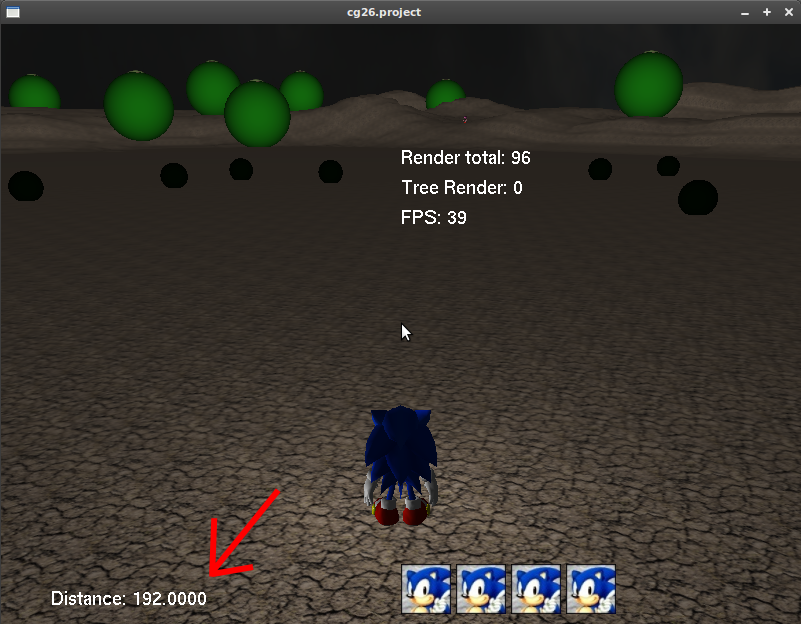
\includegraphics[width=0.7\textwidth]{images/radar.png}}
                 \caption{Radar.}
                 \label{fig:prototype}
\end{figure}

Eis o código que apresenta a informação no ecrã, usando a perspectiva ortogonal para utilizar o plano do ecrã como um ambiente 2D:

\begin{lstlisting}[caption=Perspectiva Ortogonal]
namespace ChangeMode {

	void setOrthographicProjection() {
		glMatrixMode(GL_PROJECTION);
		glPushMatrix();
		glLoadIdentity();
		gluOrtho2D(0, g_win_w, 0, g_win_h);
		glMatrixMode(GL_MODELVIEW);
		glLoadIdentity();
		glDisable(GL_LIGHTING);
	}


	void resetPerspectiveProjection() {
		glMatrixMode(GL_PROJECTION);
		glPopMatrix();
		glMatrixMode(GL_MODELVIEW);
		glLoadIdentity();
		glEnable(GL_LIGHTING);
	}

}
\end{lstlisting}

Estes dois métodos permitem alternar entre a perspectiva normal e a perspectiva ortogonal, usada para escrever no ecrã em formato 2D.

\begin{lstlisting}[caption=Render do Radar]
void Radar::render() {
	char *string = new char[50];
	switch (g_player->state) {
		case GAME_ON:
			if (g_keys->keys_left == 0)
				sprintf(string, "All keys catched. GO FOR THE TOILET!");
			else if (dist > range)
				sprintf(string, "Distance: > 500 meters");
			else
				sprintf(string, "Distance: %d", (int) dist);
			break;
		case GAME_OVER:
			sprintf(string, "GAME OVER. YOU LOST!");
			break;
		case GAME_WIN:
			sprintf(string, "YOU WON! Press ESC to quit");
			break;
	}

	int len, i;
	len = strlen(string);
	
	ChangeMode::setOrthographicProjection();
	glPushMatrix();
	glLoadIdentity();

	glColor3f(1.0f, 1.0f, 1.0f);
	glRasterPos2i(screen_coords->x, screen_coords->y);
	
	for (i = 0; i < len; i++) {
		glutBitmapCharacter(GLUT_BITMAP_HELVETICA_18, string[i]);
	}
	glPopMatrix();
	ChangeMode::resetPerspectiveProjection();
}
\end{lstlisting}

Esta função utiliza a perspectiva ortogonal e a função \textbf{glutBitmapCharacter} para desenhar caracteres no ecrã, a partir de uma string que informa o jogador do estado actual do radar.
